
\section{Breakup}
\newcommand{\zbx}{Z^{(b)}_x(\xi,\vecr_x)}
%\newcommand{\images}{images}
\newcommand{\bx}{\mathbf{x}}
\newcommand{\by}{\mathbf{y}}
%-------------------------------

%-----------------------------
\subsection{The CDCC method}

\slide{}
\begin{center}
\psframebox[fillcolor=green!10,linecolor=blue,framearc=0.1,fillstyle=solid,framesep=5pt]{
Inclusion of breakup channels: the CDCC method
}%psframe
\end{center} 
\end{frame}




%------------------------------------
\slide{Breakup modelspace}

\begin{figure}{\par \resizebox*{0.2\textwidth}{!}
{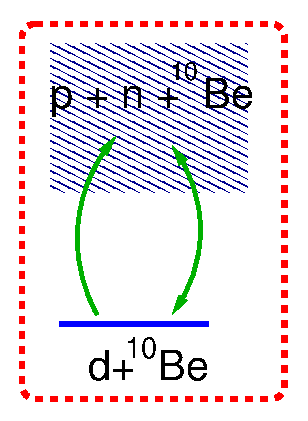
\includegraphics{\images/be10d_modelspace_bu.eps}} \par}
\end{figure}

\vspace{1cm}

\begin{center}
\psframebox[fillcolor=yellow!40,fillstyle=solid,framearc=0.2]{
\parbox{0.8\columnwidth}{%
\ding{43}{\em \small We want to include explicitly in the modelspace the breakup channels of the projectile or target.}
}%parbox
}%psframe
\end{center}

%\ding{43} In a transfer calculation, the modelspace will contain states belonging to different mass partitions.


\end{frame}



% ----------------------------------------------------------------------------------------------------
\slide{The CC method for bound states}
We need to incorporate explicitly in the Hamiltonian the internal structure of the nucleus being excited (eg.~ {\verde target}).
$$ 
\psframebox[linecolor=red,framearc=0.1]{
 H = T_R   +  h(\xi)+ V(\bR, \xi)
}
$$


\begin{itemize}
\gitem{$T_R$}: Kinetic energy for projectile-target relative motion.
\gitem{$\{\xi\}$}: Internal degrees of freedom of the target (depend on the model).
\gitem{$h(\xi)$}: Internal Hamiltonian of the target.
$$
\psframebox[linecolor=red,framearc=0.1]{
h(\xi)\phi_{n}(\xi)  =  \varepsilon_{n}\phi_{n}(\xi)
}
$$

\gitem{$V(\bR, \xi)$}: Projectile-target interaction %, eg:
% $$ V(\bR, \xi) = \sum_{i=1}^{N} V_{pi}(\br_{pi}) $$

% \pause 
% \item[] {\bf Eg.:} $^7$Li=$\alpha+t$ $\Rightarrow$ {\verde $\{\xi\} \equiv \bf r$}
% $$
% V_\mathrm{p-7Li}({\bf R}, {\bf r})= V_\mathrm{p-t}\left({\bf R} +\frac{4}{7}{\bf r}\right) 
% + 
% V_\mathrm{p-\alpha}\left({\bf R} +\frac{3}{7}{\bf r}\right)
% $$
\end{itemize}
\end{frame}





% ----------------------------------------------------------------------------------------------------
\slide{The CC method (continued): CC model wavefunction}

We expand the total wave function in a subset of internal states (the {\cal P} space):
$$
\psframebox[linecolor=red,framearc=0.1]{
\Psi^{(+)}_\mathrm{model}(\bR,\xi)=\phi_{0}(\xi)\chi_{0}(\bR)+ \sum_{n>0} \phi_{n}(\xi)\chi_{n}(\bR)  
}
$$

Boundary conditions for  the $\chi_{n}(\bR)$ (unknowns):

\begin{align*}
\chi_0^{(+)}(\bR) & \rightarrow  e^{i \bK_0 \cdot \bR}  + {\red f_{0,0}(\theta)} \frac{e^{i K_0 R}}{R} 
\quad \quad  \textrm{\blue for n=0 (elastic)} \\
\chi_n^{(+)}(\bR) & \rightarrow                           {\red f_{n,0}(\theta)} \frac{e^{i K_n R}}{R} 
\quad  \quad \quad \quad \textrm{\blue for n>0 (non-elastic)}
\end{align*}

\end{frame}





% ----------------------------------------------------------------------------------------------------
\slide{The CC method (continued): calculation of $\chi_n^{(+)}(\bR)$; the coupled equations}

\begin{itemize}
\item The model wavefunction must satisfy the Schr\"odinger equation:
$$
 [H-E]\Psi^{(+)}_\mathrm{model}(\bR,\xi)=0
$$

\item Projecting onto the internal states one gets a system of coupled-equations for the functions 
{\verde $\{\chi_{n}(\bR) \}$:}
$$
\psframebox[linecolor=red,framearc=0.1]{
\left[E-\varepsilon_{n}-T_R -V_{n,n}(\bR) \right] \chi_{n}(\bR)  = 
\sum_{n' \neq n} V_{n,n'}(\bR) \chi_{n'}(\bR) 
}%psframebox
$$


\item The structure information is embedded in the {\verde coupling potentials:}
$$
\psframebox[linecolor=red,framearc=0.1]{
V_{n,n'}(\bR) = \int   d \xi \phi_{n'}(\xi)^* V(\bR, \xi) \phi_{n}(\xi) 
}%psframebox
$$

\item[\ding{43}] {\small \em \blue $\phi_{n}(\xi)$ will depend on the structure model 
(collective, single-particle,etc).}

\end{itemize}
\end{frame}



% -------------------------------------------------------------------------------------------------
\slide{Choice of structure model: the few-body (cluster) case}


\bc
\column{0.45\linewidth}
\begin{center}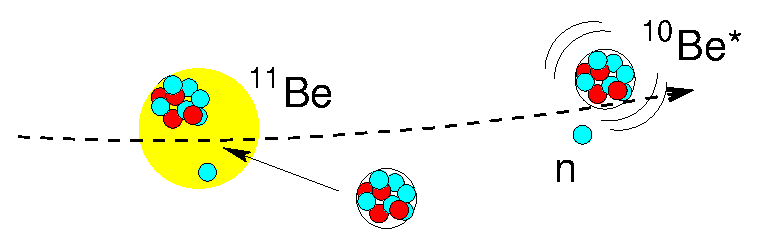
\includegraphics[width=0.85\columnwidth]{\images/be11t_mic.eps}\end{center}
\begin{center} $${\cal V}_{pt} = \sum_{ij} V_{ij}(\br_{ij})$$  \end{center}

\column{0.15\linewidth}
\begin{center}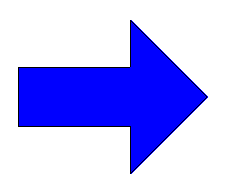
\includegraphics[width=0.7\columnwidth]{\images/arrow-blue.eps}\end{center}
\column{0.45\linewidth}
\begin{center}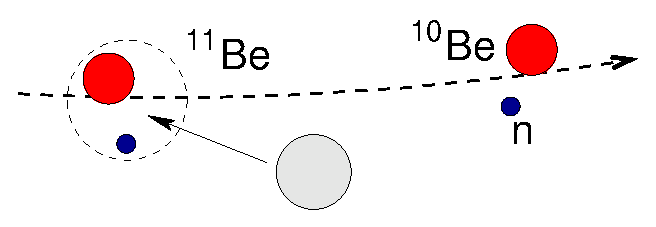
\includegraphics[width=0.85\columnwidth]{\images/be11t_inert.eps}\end{center}
\begin{center}$${\cal V}_{pt} = U_{ct}(\br_{ct}) + U_{nt}(\br_{nt})$$\end{center}

\ec

\bi

\bigskip

\item Effective {\blue three-body} Hamiltonian:
$$
\psframebox[linecolor=red,fillcolor=orange!10,fillstyle=solid,framearc=0.2]{
H = T_\bR   +  h_r(\br) + U_{ct}(\br_{ct}) + U_{nt}(\br_{nt})
}%psframe
$$ 


\item $U_{ct}(\br_{ct})$, $U_{nt}(\br_{nt})$ are optical potentials describing fragment-target elastic scattering (eg.~target excitation is treated effectively, through absorption) 


\ei

\end{frame}


% ----------------------------------------------------------------------------------
\slide{Inelastic scattering in a few-body model}

\begin{itemize}
\gitem{Some nuclei allow a description in terms of two or more clusters:} \\ 
d=p+n,  \nuc{6}{Li}=$\alpha$+d, \nuc{7}{Li}=$\alpha$+\nuc{3}{H}. 

\gitem{Projectile-target interaction:}
 $$ 
 V(\bR,\xi) \equiv V(\bR,\br)= U_{1}(\br_1) + U_2(\br_2)
 $$


\gitem{Transition potentials:}
 $$
\psframebox[linecolor=red,framearc=0.1]{
 V_{n,n'}(\mathbf{R})=\int d\mathbf{r}\phi_{n}^{*}(\br)\left[U_{1}(\br_1) + U_2(\br_2)\right] \phi_{n'}(\br)
}
$$ 

\pause 

%\parbox{0.7\textwidth}{
\psframebox[fillcolor=green!10,linecolor=blue,framearc=0.1,fillstyle=solid]{
\begin{minipage}{.55\textwidth}
%\begin{columns}
%\column{0.3\textwidth}
\textcolor{blue}{Example:} $^7$Li=$\alpha$+t
 $$
 \br_\alpha= \bR - \frac{m_t}{m_\alpha+m_t} \br ;
 \quad 
 \br_t= \bR + \frac{m_\alpha}{m_\alpha+m_t}\br
 $$
{\blue Internal states:} (two-body cluster model)
 $$[T_\br + V_{\alpha-t}(\br) - \varepsilon_n ]\phi_n(\br)=0$$
\end{minipage}
%\column{0.3\textwidth}
\begin{minipage}{.35\textwidth}
\begin{center}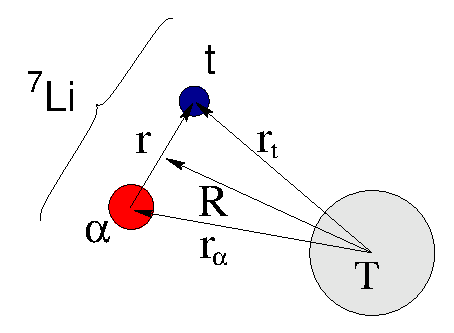
\includegraphics[width=0.7\columnwidth]{\images/li7t_coord.eps}\end{center}
%\end{columns}
\end{minipage}
%}%parbox
}%psframe


\end{itemize}

\end{frame}



% ----------------------------------------------------------------------------------
\slide{Example: \nuc{7}{Li}($\alpha$+$t$) +\nuc{208}{Pb} at 68 MeV}

%{\bf Example:} \nuc{7}{Li}($\alpha$+$t$) +\nuc{208}{Pb} at 68 MeV {\verde (Phys. Lett. 139B (1984) 150)}: 
%\ding{43}    Uses $\alpha$+t model for \nuc{7}{Li}
%$$
%V_{n,n'}(\bR)=\int d\br \phi_{n}^{*}(\br)
%\left[V_\mathrm{\alpha}(\br_{\alpha}) + V_\mathrm{t}(\br_{t}) \right]
%\phi_{n'}(\br)  ; \quad  n=0,1
%$$

\ding{233} CC calculation with 2 channels (3/2$^-$, 1/2$^-$)  {\verde (Phys. Lett. 139B (1984) 150)}
\begin{columns}
\column{0.4\textwidth}
\begin{center}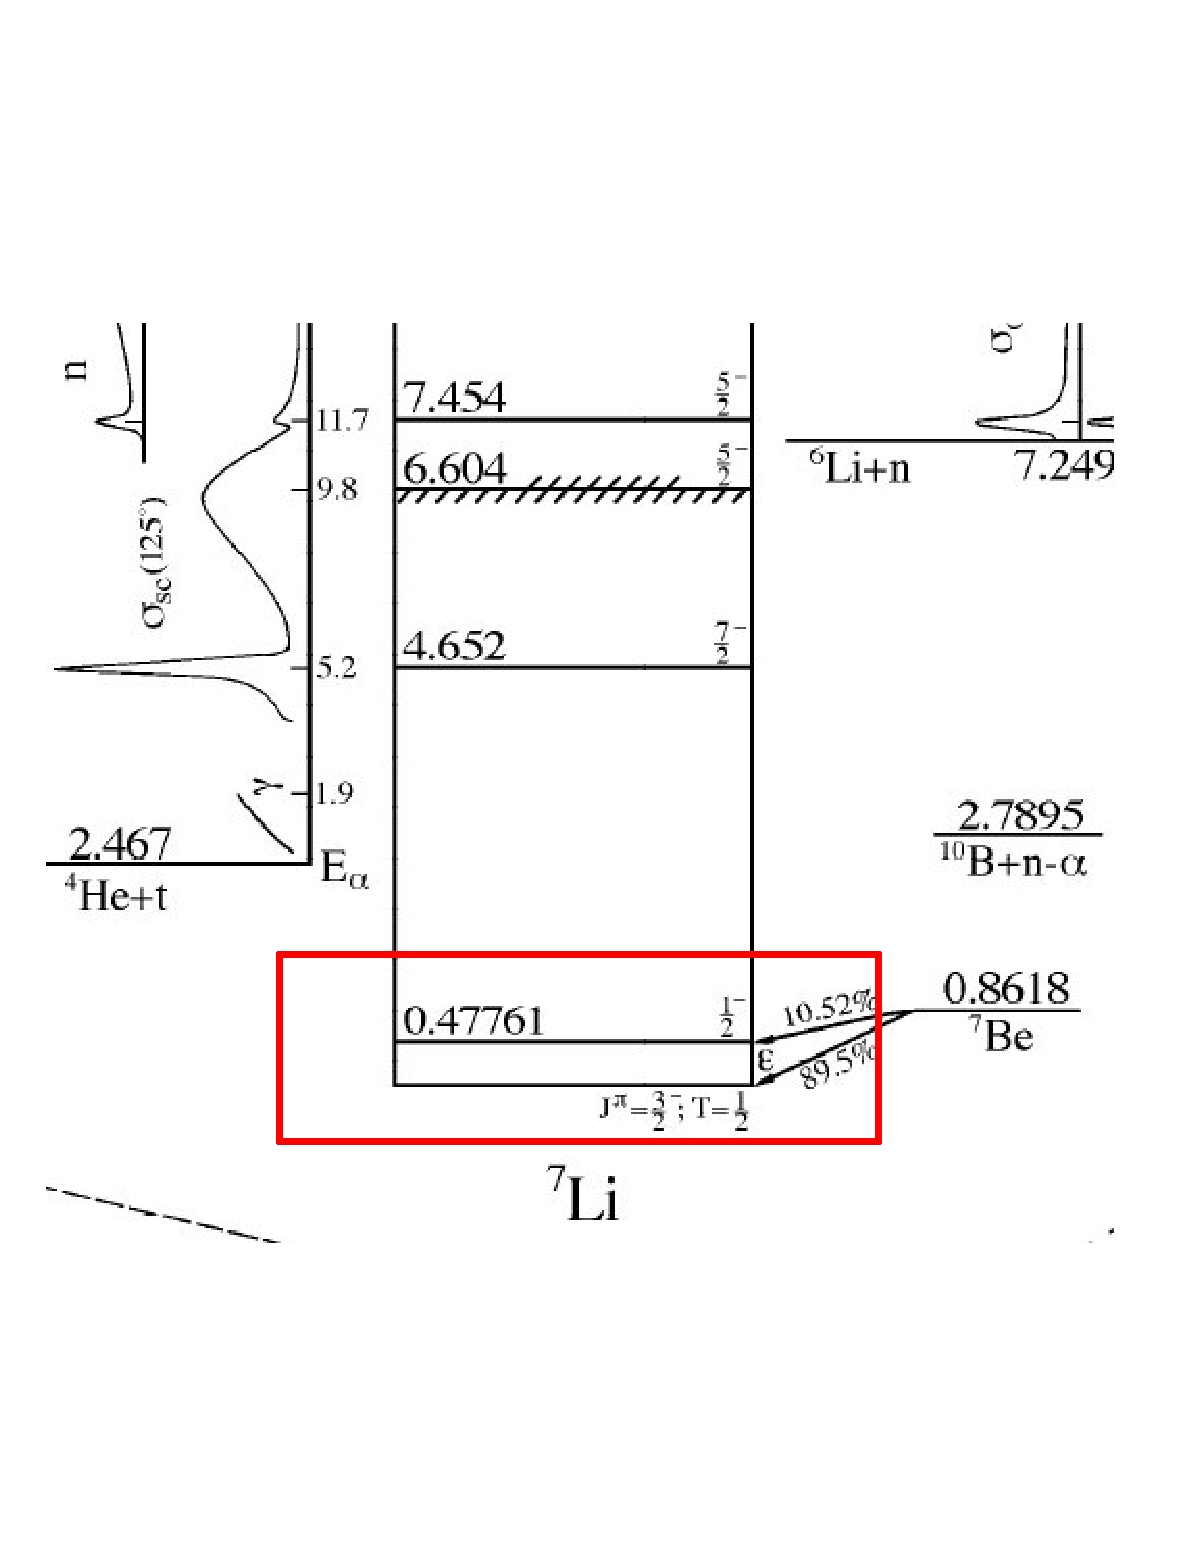
\includegraphics[height=6.0cm]{\images/li7spectrum2.eps} \end{center}
\column{0.5\textwidth}
\begin{center}
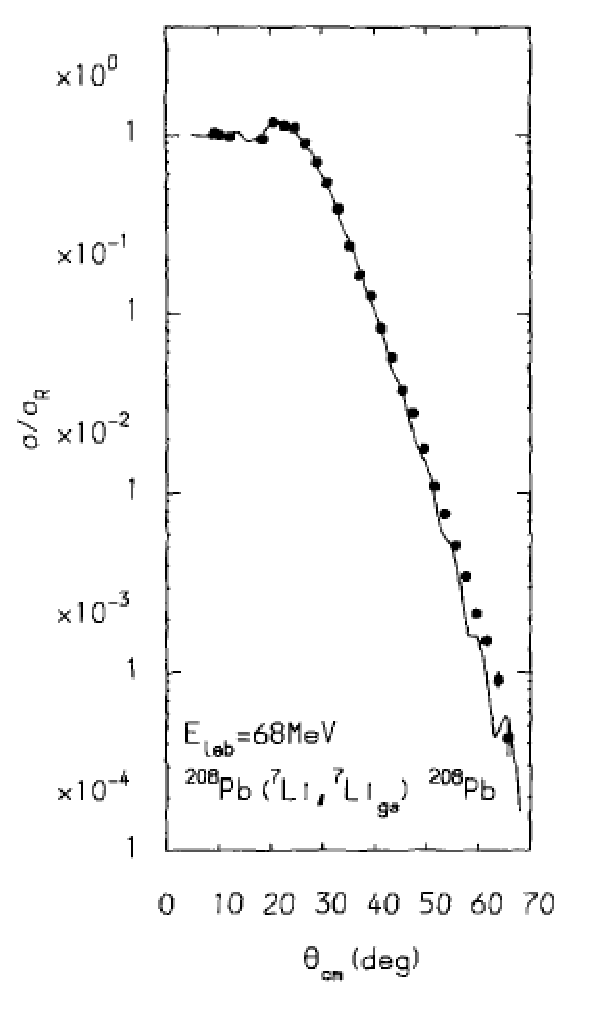
\includegraphics[height=5.5cm]{\images/li7pb_e70_el.eps} 

\includegraphics[height=5.5cm]{\images/li7pb_e70_inel.eps} 
\end{center}
\end{columns}
\end{frame}









%\subsection{The importance of the coupling to breakup channels}


% --------------------------------------------------------------------------------------
\slide{Application of the CC method to weakly-bound systems}


{\bf Example:}  {\blue Three-body calculation (p+n+\nuc{58}{Ni}) with Watanabe potential:}
$$
V_{dt}(\vecR)=\int d \vecr  \phi^*_\mathrm{gs}(\vecr) \left\{ V_{pt}(\br_{pt})  + V_{nt}(\br_{nt}) \right\}
 \phi_\mathrm{gs}(\vecr)
$$

\begin{columns}
\column{0.5\textwidth}
\begin{figure}{\par \resizebox*{0.8\textwidth}{!}
{\includegraphics{\images/dni_e80_1chan.eps}} \par}
\end{figure}
\column{0.4\textwidth}
\begin{center}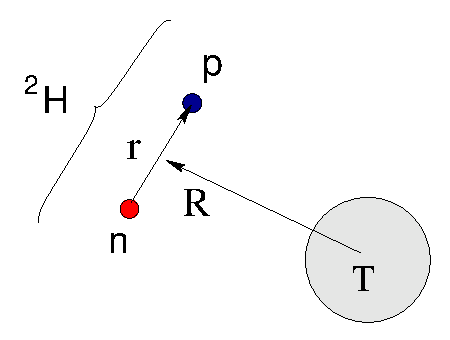
\includegraphics[height=2.5cm]{\images/dpb_coor.eps}\end{center}
\end{columns}


\ding{43}{\em \blue \small Three-body calculations omitting breakup channels fail to describe 
the experimental data.}
\end{frame}



% -------------------------------------------------------------------------------------------------
\slide{Bound versus scattering states}

\begin{columns}
\column{0.5\textwidth}
 \begin{figure}{\par \resizebox*{0.9\textwidth}{!}
 {\includegraphics{\images/deut2}} \par}
 \end{figure}
\column{0.5\textwidth}
Continuum wavefunctions: 
\bigskip

\psframebox[fillcolor=lightgreen,linecolor=blue,framearc=0.1,fillstyle=solid,framesep=-5pt]{
\parbox{0.9\columnwidth}{
$$ 
\varphi_{k,\ell jm}(\br) = {u_{k, \ell j} (r) \over r} [Y_{\ell}(\hat{r}) \otimes \chi_s  ]_{jm} 
$$
$$ 
\varepsilon=\frac{\hbar^2 k^2}{2 \mu} 
$$
}%parbox
}%psframe
\end{columns}

\pause
\vspace{0.5cm}

{\brick Unbound states are not suitable for CC calculations:} \\
\begin{itemize}
\item They have a continuous (infinite) distribution in energy.
\item Non-normalizable: $\langle u_{k,\ell s j}(r) | u_{k',\ell s j}(r) \rangle \propto \delta(k-k')$ 
\end{itemize}

\bigskip
\centering{ {\blue SOLUTION} $\Rightarrow$ {\blue continuum discretization}}

\end{frame}
% ------------------------------------------------------------------------------------------------


% -------------------------------------------------------------------------------------------------
\slide{The role of the continuum in the scattering of weakly bound nuclei}

\begin{itemize}

\item Continuum discretization method proposed  by G.H.~Rawitscher {\verde [ PRC9, 2210 (1974)]} and Farrell, Vincent and 
Austern {\verde [Ann.Phys.(New York) 96, 333 (1976)]}.
 \begin{figure}{\par \resizebox*{0.9\textwidth}{!}
 {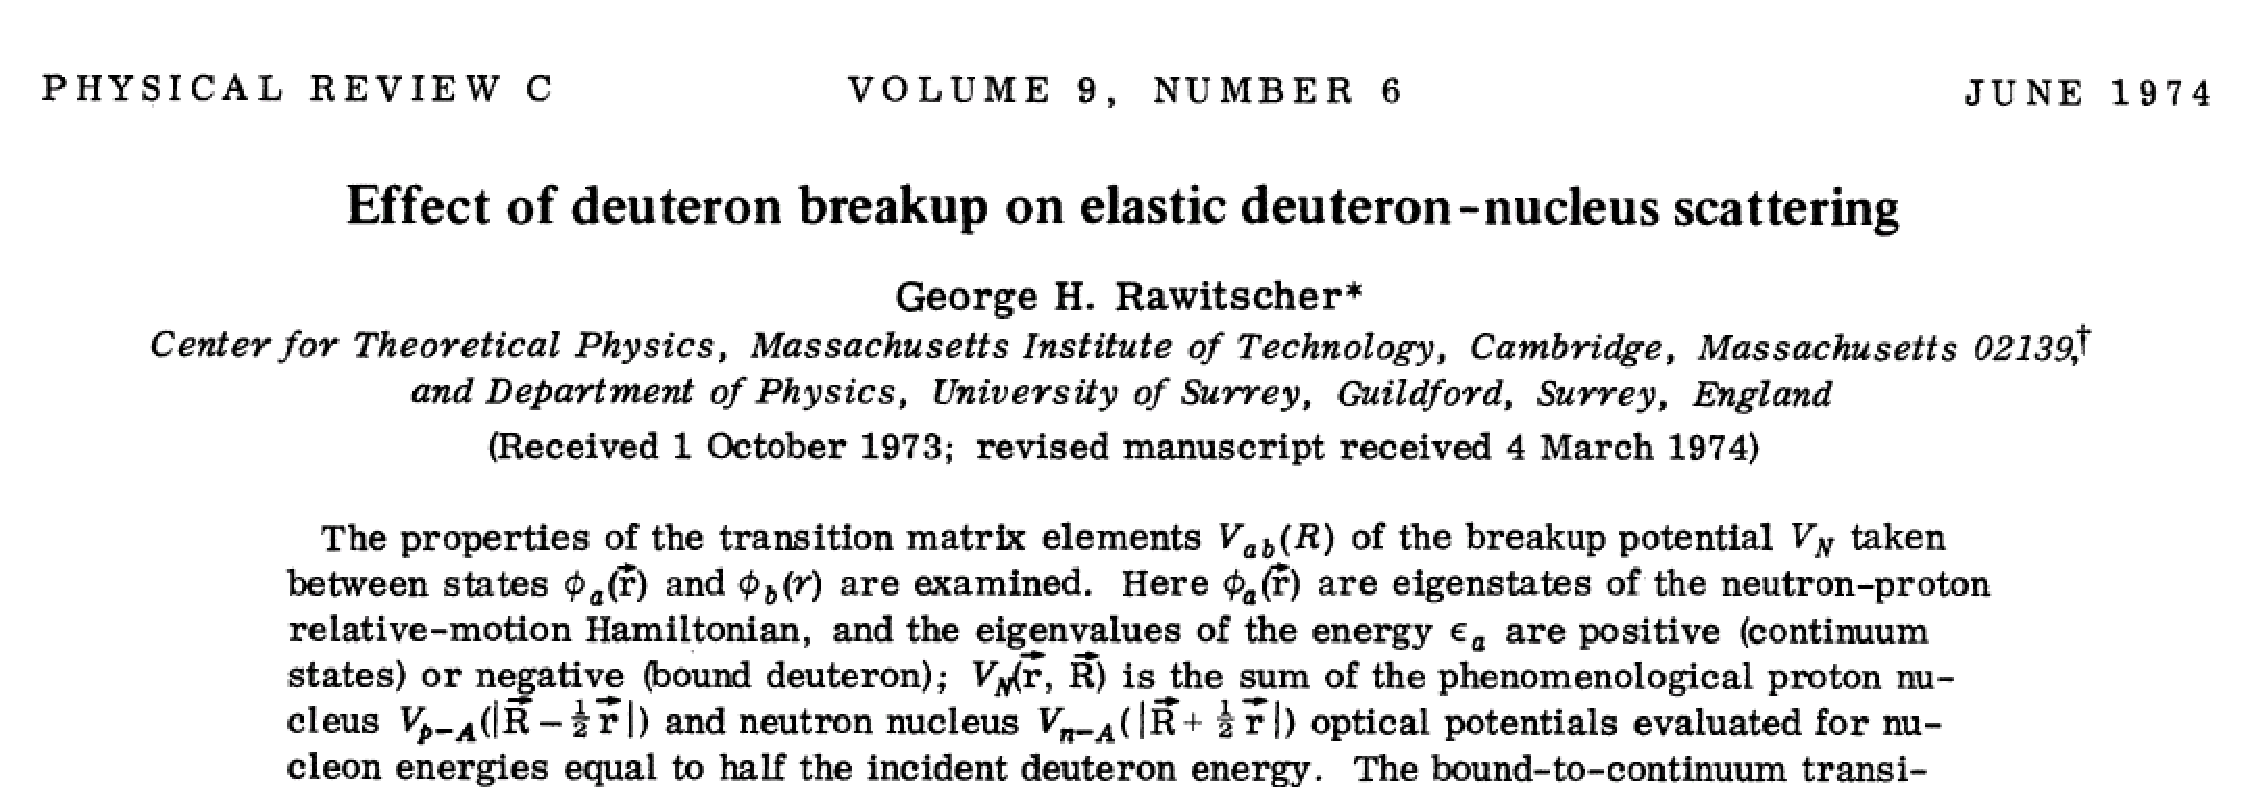
\includegraphics{\images/rawitscher.eps}} \par}
 \end{figure}


\item Full numerical implementation  by Kyushu group (Sakuragi, Yahiro, Kamimura, and co.): {\verde Prog.~Theor.~Phys.(Kyoto) 68, 322 (1982)}

\end{itemize} 
\end{frame}



% -------------------------------------------------------------------------------------------------
\slide{Continuum discretization for deuteron scattering}
%-----------------------------------------------------
\vspace{0.5cm}

%{\brick CDCC method} $\rightarrow$ continuum discretization: 

%{\blue Example:} discretization of the deuteron continuum in terms of energy bins.

%\begin{columns}
%\column{0.4\textwidth}
 \begin{figure}{\par \resizebox*{0.55\textwidth}{!}
 {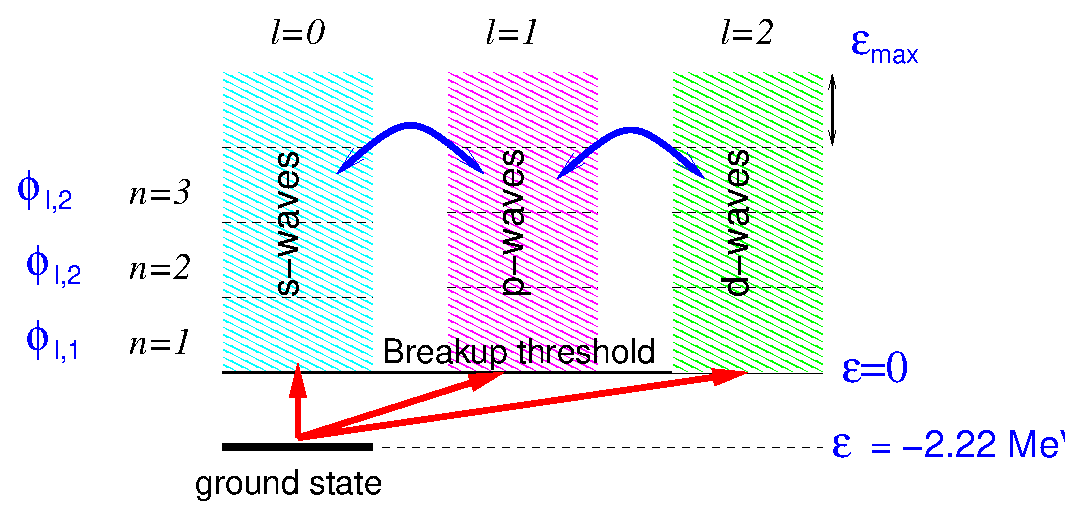
\includegraphics{\images/cdcc_deut.eps}} \par}
 \end{figure}
%\column{0.6\textwidth}
 \begin{itemize}
 \small
 \item[\ding{233}] Select a number of angular momenta ({\blue $\ell=0,\ldots,\ell_\mathrm{max}$}).
 \item[\ding{233}] For each $\ell$, set a maximum excitation energy {\blue $\varepsilon_\mathrm{max}$}.
 \item[\ding{233}] Divide the interval {\blue $\varepsilon=0-\varepsilon_\mathrm{max}$} in a set of sub-intervals ({\em \blue bins}).
  \item[\ding{233}] For each {\blue bin}, calculate a representative wavefunction. 
 \end{itemize}
%\end{columns}


\end{frame}
% --------------


% -------------------------------------------------------------------------------------------------
\slide{CDCC formalism: construction of the bin wavefunctions}

%\vspace{0.5cm}

{\blue Bin wavefunction:} $$\varphi^{[k_1,k_2]}_{\ell jm}(\br) =  {u^{[k_1,k_2]}_{\ell j}(r) \over r} [Y_{\ell}(\hat{r}) \otimes \chi_s  ]_{jm} 
\quad 
\quad 
[k_1,k_2] = \textrm{bin interval}
$$


\vspace{0.24cm}
\begin{columns}
\column{0.5\textwidth}
$$
\psframebox[linecolor=red,framearc=0.1]{
 u^{[k_1,k_2]}_{\ell sjm} (r) = \sqrt {\frac{2 }{\pi N}} ~~
            \int _ {k _ 1} ^ {k _ 2} w(k) u _{k,\ell sj} (r) dk
}%psfram
$$
\column{0.5\textwidth}
\begin{itemize}
\setlength{\itemsep}{0pt}
\item {\blue $k$}: linear momentum
\item {\blue $u _{k,\ell sj}(r)$}: scattering states (radial part)
\item {\blue $w(k)$}: weight function 
\end{itemize}
\end{columns}

\nccurve[linecolor=magenta,angleA=-90,angleB=155]{->}{F1}{T1}

\vspace{+0.2cm}

 \begin{figure}{\par \resizebox*{0.42\textwidth}{!}
 {\includegraphics{\images/wfbin.eps}} \par}
 \end{figure}

\end{frame}
% ------------------------------------------------------------------------------------------------



\begin{comment}

% --------------------------------------------------------------------------------------
\slide{Inclusion of the continuum in CC calculations: continuum discretization}

%\hspace{3.5cm}\rnode{A}{\psshadowbox[fillcolor=yellow,linecolor=black,framearc=0.2]{\blue Quantum Hamiltonian}}

\begin{center}\psshadowbox[fillcolor=yellow,linecolor=black,framearc=0.2]{\blue Quantum Hamiltonian}\end{center}


\vspace{1cm}
\begin{columns}
\column{0.5\linewidth}
%\hspace{0.5cm}\rnode[linecolor=red]{B1}
\begin{center}
{\psframebox{\parbox{3cm}{{\bf \verde Bound states}\\ - Discrete \\ - Finite \\ - Normalizable}}}
\end{center}
\column{0.5\linewidth}
\begin{center}
%\hspace{0.5cm}\rnode[linecolor=red]{B2}
{\psframebox{\parbox{4cm}{{\bf \verde Unbound states} \\ - Continuous \\ - Infinite \\ - Non-normalizable}}}
\end{center}
\end{columns}

%\ncline{->}{A}{B1}
%\ncline{->}{A}{B2}
%\nccurve[linecolor=red,angleA=-90,angleB=90]{->}{A}{B1}
%\nccurve[linecolor=red,angleA=-90,angleB=90]{->}{A}{B2}

\vspace{1cm}

{\bf \brick Continuum discretization:} represent the continuum by a finite set of square-integrable states

\begin{center}
\begin{tabular}{lcl}
%\small
{\bf \verde {\em True} continuum} & $\to$ & {\bf \verde Discretized continuum } \\
{Non normalizable}  &  $\to$ & {Normalizable} \\
{Continuous}         & $\to$ & {Discrete }
\end{tabular}
\end{center}
%}

\end{frame}
\end{comment}


\begin{comment}
% -------------------------------------------------------------------------------------------------
\slide{CDCC formalism}

\vspace{0.5cm}

%{\brick CDCC method} $\rightarrow$ continuum discretization: 
Coupled-Channels + Continuum discretization $\Rightarrow$ Continuum-Discretized Coupled-Channels (CDCC)!


{\brick Example:} discretization of the deuteron continuum in terms of energy bins.


 \begin{figure}{\par \resizebox*{0.65\textwidth}{!}
 {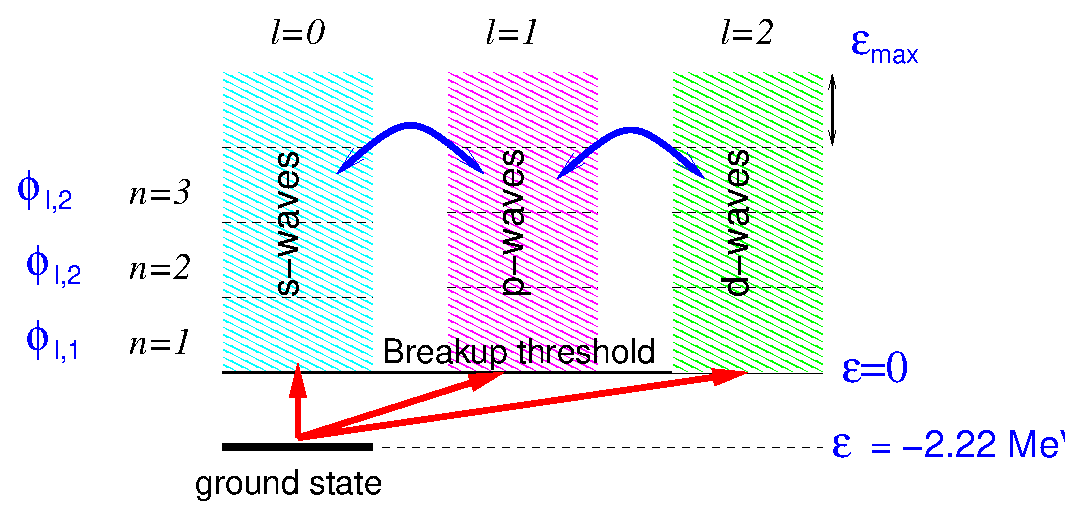
\includegraphics{\images/cdcc_deut}} \par}
 \end{figure}

\end{frame}
\end{comment}



\begin{comment}
% -------------------------------------------------------------------------------------------------
\slide{CDCC formalism: construction of the bin wavefunctions}

%\vspace{0.5cm}

{\brick Bin wavefunction:} 

\begin{center}
\psframebox[linecolor=red,framearc=0.1,framesep=0.0cm]{
\parbox{7.0cm}{
\begin{equation} 
\nonumber
{  u_{\ell sj,n} (r) = \sqrt {\frac{2 }{\pi N}} ~~
            \int _ {k _ 1} ^ {k _ 2} w(k) u _{\ell sj,k} (r) dk}
\end{equation}
}}%parbox
\end{center}

\begin{itemize}
\setlength{\itemsep}{0pt}
\item {\brick $k$}: linear momentum
\item {\brick $u _{\ell sj,k}$}: scattering states (radial part)
\item {\brick $w(k)$}: weight function 
\end{itemize}

\vspace{-0.2cm}

 \begin{figure}{\par \resizebox*{0.42\textwidth}{!}
 {\includegraphics{\images/wfbin.eps}} \par}
 \end{figure}

\end{frame}
% ------------------------------------------------------------------------------------------------
\end{comment}





% -------------------------------------------------------------------------------------------------
\slide{CDCC formalism for deuteron scattering}
% $\bullet$ Radial wavefunctions: 

%{\brick CDCC equations for radial wavefunctions:}

\begin{itemize}
\bc
\column{0.65\linewidth}
\gitem{Hamiltonian:}  $H = T_\bR   +  h_r(\br) + V_{pt}(\br_{pt}) + V_{nt}(\br_{nt})$ 

\gitem{Model wavefunction:}
 $$\Psi^{(+)}(\bR,\br)=\phi_{gs}(\br)\chi_{0}(\bR)+ \sum_{n>0}^{N} \phi_{n}(\br) \chi_{n}(\bR)$$

\column{0.35\linewidth}
\begin{figure}{\par \resizebox*{0.75\textwidth}{!}
 {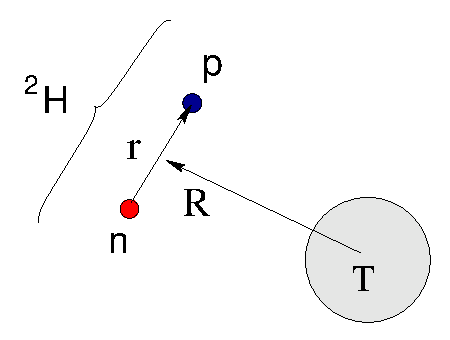
\includegraphics{\images/dpb_coor}} \par}
 \end{figure}
\ec

\gitem{Coupled equations:} $[H-E]\Psi(\bR,\br)=0$
$$
\psframebox[linecolor=red,framearc=0.1]{
\left[E-\varepsilon_{n}-T_R -V_{n,n}(\bR) \right] \chi_{n}(\bR)  = 
\sum_{n' \neq n} V_{n,n'}(\bR) \chi_{n'}(\bR) 
}%psframebox
$$

%-----------------
% Radial equations
% ----------------
% $$
% \psframebox[linecolor=red,framearc=0.1,framesep=2mm]{
%  \left [ 
% - \frac{\hbar^2 }{2 \mu} ~ \left ( \frac{d^2 }{ dR^2} - \frac{L(L+1)} {R^2} \right )
% + \epsilon_n - E \right ]
% f _ {\alpha J} (R)  + \sum _ {\alpha '} 
% i ^ {L ' - L} ~ V^J _{\alpha:\alpha'}(R)  f_{\alpha' J} (R) =0 
% }
% $$
% {\brick $\alpha$}= $\{L,\ell,s,j,n\}$ 


\gitem{Transition potentials:}
$$
%\psframebox[linecolor=red,framearc=0.2,framesep=2mm]{
V_{n;n^\prime}(\vecR) = 
\int d \vecr  \phi_n^{*}(\vecr)
	\left[ V_{pt} (\vecR +\frac{\vecr}{2}) + V_{nt} (\vecR-\frac{\vecr}{2})\right] 
 \phi_{n^\prime}(\vecr) 
%}
$$

\end{itemize}

\end{frame}
% -------------------------------------------------------------------------------------------------


% ------------------------------------------------------------------------------------------------
\slide{Application of the CDCC formalism: d+ $^{58}$Ni}

%\psframebox[fillcolor=green!15,linecolor=blue,framearc=0.1]{
\begin{center}\small Coupled-Channels + Continuum discretization \end{center}
%}%
\begin{center}$\Downarrow$ \end{center}
\begin{center}
\psframebox[fillcolor=green!15,linecolor=blue,framearc=0.1]{
\small Continuum-Discretized Coupled-Channels (CDCC) 
}%psframe
\end{center}

\begin{columns}
\column{0.5\textwidth}
\begin{figure}{\par \resizebox*{0.8\textwidth}{!}
    {\includegraphics{\images/dni_e80_kd.eps}} \par}
\end{figure}
\column{0.5\textwidth}
\begin{center}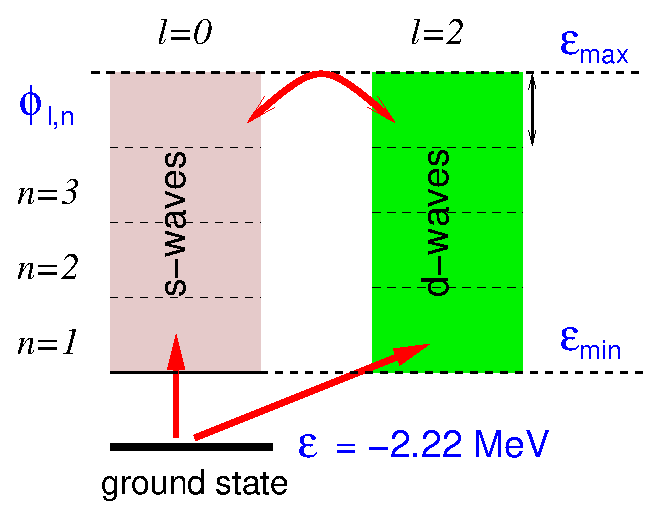
\includegraphics[width=0.75\textwidth]{\images/cdcc_deut_sd.eps} \end{center}

\end{columns}

% \ding{43} No continuum $\Rightarrow$ retain only the Watanabe potential: 
% $$
% V_{00}(\vecR)=\int d \vecr  \phi_\mathrm{gs}(\vecr) \left( V_{pt}  + V_{nt}\right)
%  \phi_\mathrm{gs}(\vecr)
% $$

\bigskip

\ding{43}{\it \small Coupling to breakup channels has a important effect on the reaction dynamics}

\end{frame}





% --------------------------------------------------------------------------------------
\slide{Application of the CDCC method: \nuc{6}{Li} and \nuc{6}{He} scattering}

\begin{itemize}
\item[\ding{43}]{\verde The CDCC has been also applied to nuclei with a cluster structure:}
\item \nuc{6}{Li}=$\alpha$ + d ~~~~ ($S_{\alpha,d}$=1.47~MeV)
\item \nuc{11}{Be}=\nuc{10}{Be} + n ($S_n$=0.504~MeV)
\end{itemize}

\medskip
\bc
\column{0.5\linewidth}
\begin{figure}{\par \resizebox*{0.85\textwidth}{!}
{\includegraphics{\images/li6ca_el_cdcc.eps}} \par}
\end{figure}
\column{0.5\linewidth}
\begin{figure}{\par \resizebox*{0.85\textwidth}{!}
{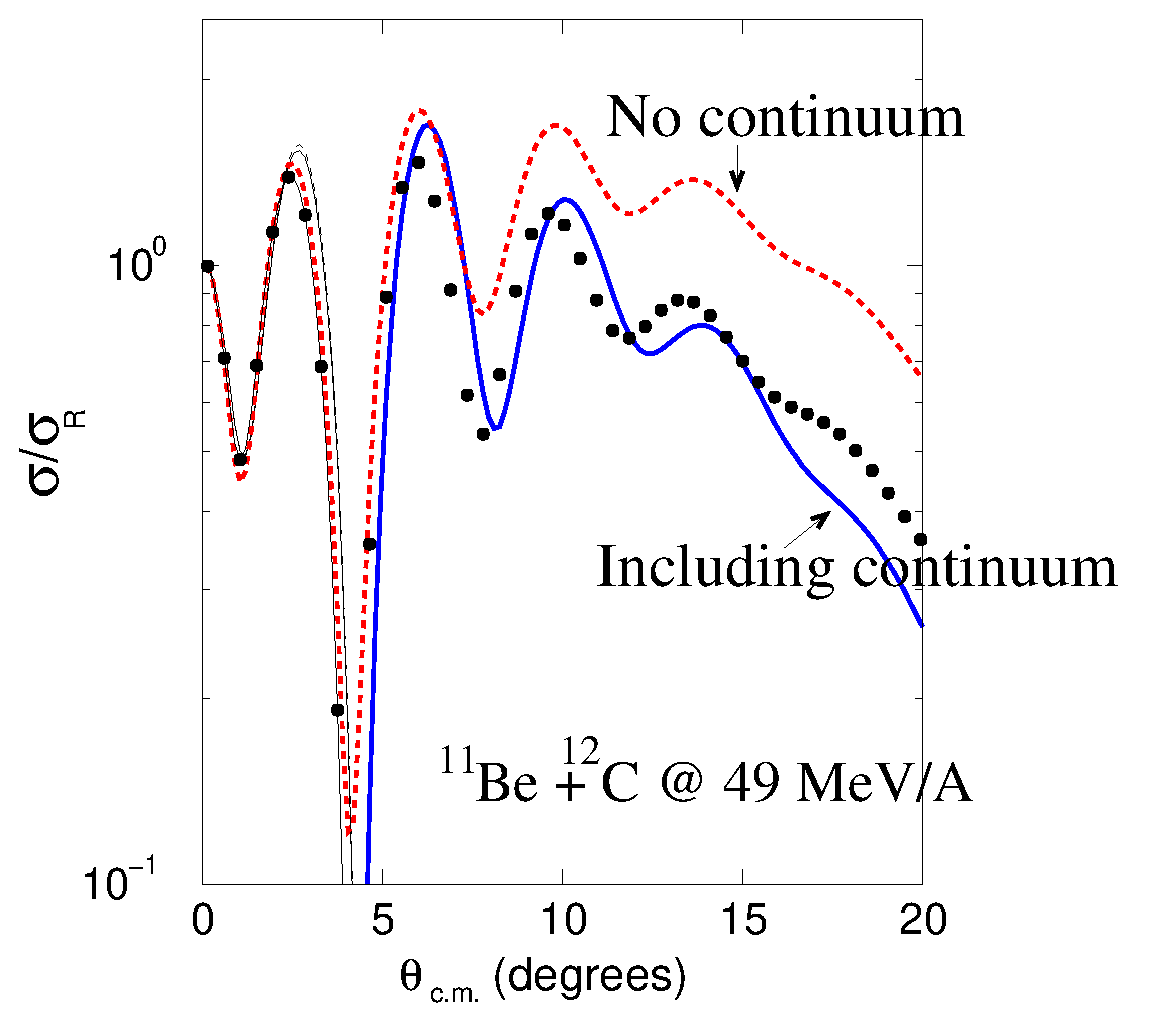
\includegraphics{\images/BeC.eps}} \par}
\end{figure}
\ec

%\pause
%\ding{43} {\verde \em \small In Fraunhofer scattering the presence of the continuum produces a reduction of the elastic  cross section} 

\end{frame}



\begin{comment}
% ---------------------------------------------------------------------------------------------------
\begin{wideslide}[toc=,bm=] {Extension to 3-body projectiles}
%\onslide*{2}{
\begin{itemize}
\item[\ding{43}]{\verde The CDCC has been recently extended to 3-body projectiles:}
\item {\bf Eg:} \nuc{6}{He}=$\alpha$ + n + n  \quad (M.Rodr\'{\i}guez-Gallardo et al,PRC 77, 064609 (2008))
\end{itemize}


\begin{figure}{\par \resizebox*{0.4\textwidth}{!}
  {\includegraphics{\images/he6pb_e27_el.eps}} \par}
  \end{figure}
%}%onslide
\pause 
\ding{43} {\verde \em \small In Fresnel scattering the coupling to the continuum supresses the interference peaks} 
\end{frame}
% --------------------------------------------------------------------------------------------------
\end{comment}






\begin{comment}
% ---------------------------------------------------------------------------------------------------
\slide{The importance of transfer/breakup channels}

\begin{itemize}
\item For ``normal'' nuclei, the elastic channel is dominant. 
\item For weakly-bound nuclei, transfer/breakup channels become very important.
\end{itemize} 

{\bf Example:} $\alpha$ particles arising in \nuc{6}{He}+\nuc{208}{Pb}

\begin{figure}{\par \resizebox*{0.40\textwidth}{!}
{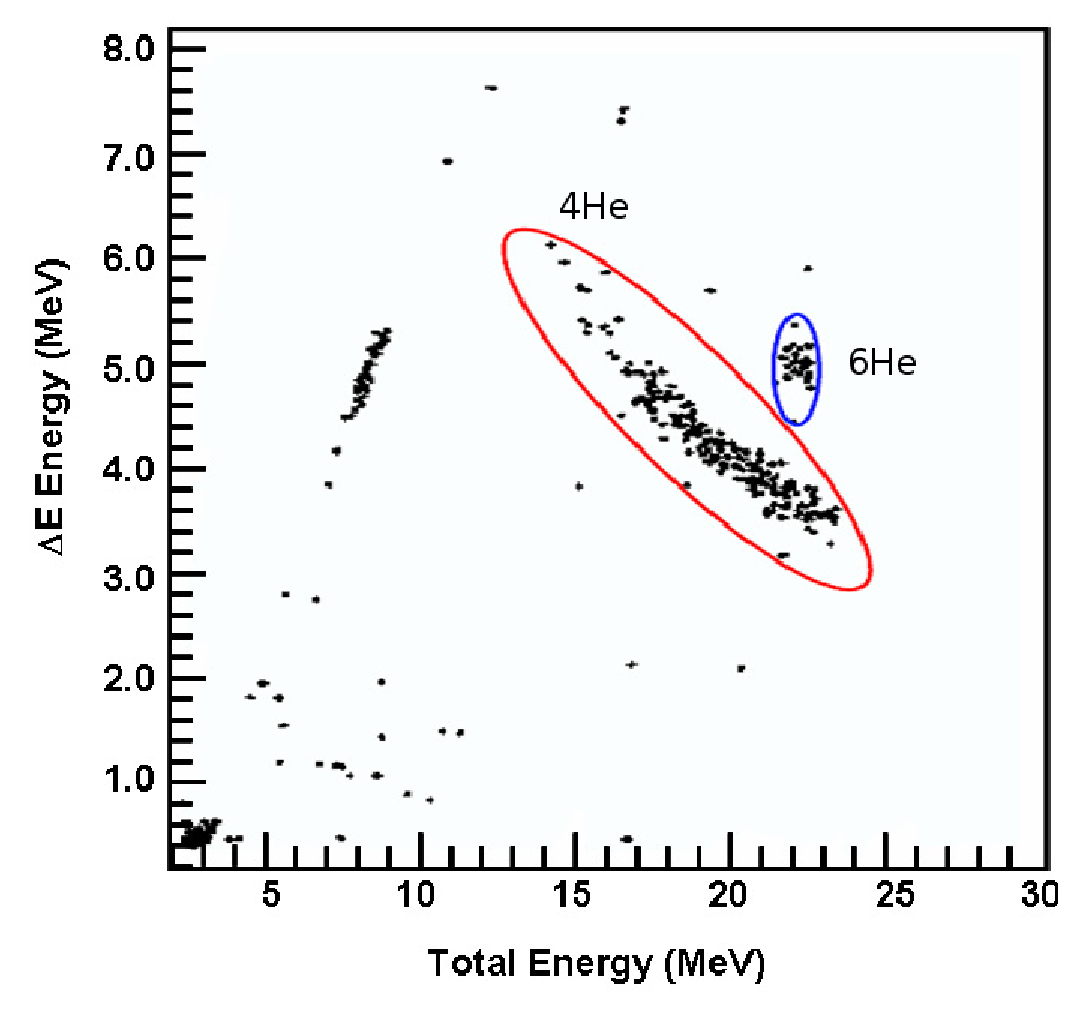
\includegraphics{\images/bidim-22MeV-new2.eps}} \par}
\end{figure}

\end{frame}
\end{comment}






%%%%%%%%%%%%%%%%%%%%%%%%%%%%%%%%%%%%%%%%%%%%%%%%%%%%%%%%%%%%%%%%%%%%%%%%%%%%%%%%%%%%%%%%%%%%%%%%%%%%%%%%%





%-----------------------------------------------------------------------------------------------------
\subsection{Recent extensions of the CDCC method}
%-----------------------------------------------------------------------------------------------------
%\slide{}
%\begin{center}
%\psframebox[fillcolor=green!10,linecolor=blue,framearc=0.1,fillstyle=solid,framesep=5pt]{
%Recent extensions of the CDCC method
%}%psframe
%\end{center} 
%\end{frame}

% ---------------------------------------------------------------------------------------------------
\slide{Extension to 3-body projectiles}

\begin{figure}{\par \resizebox*{0.4\textwidth}{!}
  {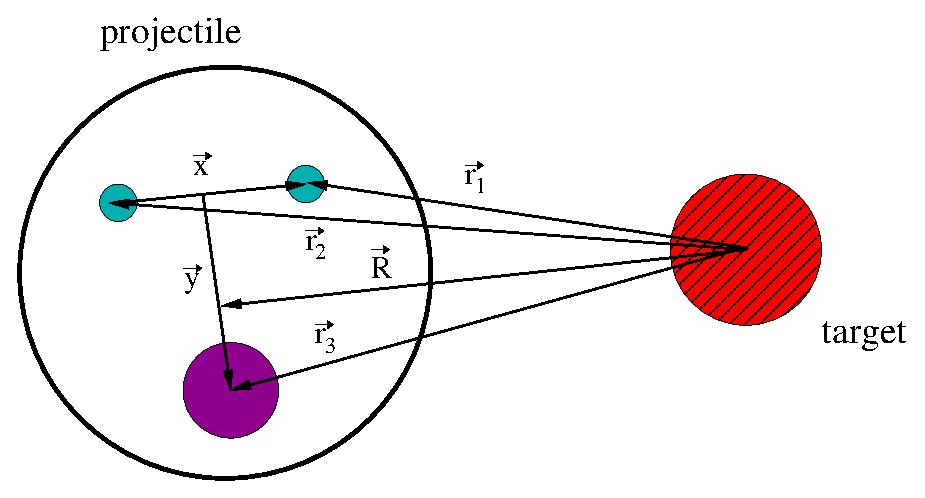
\includegraphics{\images/4c.eps}} \par}
\end{figure}


To extend the  CDCC formalism, one needs to evaluate the new coupling potentials:
$$
\psframebox[linecolor=red,framearc=0.2,framesep=1mm]{
V_{n;n^\prime}(\vecR) = 
\int d \vecr  \, \phi_n^{*}(\bx,\by)
	\left\{ V_{nt} (\br_{1}) + V_{nt} (\br_{2})  + V_{\alpha t} (\br_{3}) \right\}
 \phi_{n^\prime}(\bx,\by) 
}
$$
\ding{43} $\phi_n(\bx,\by)$ three-body WFs for bound and continuum states: hyperspherical coordinates, Faddeev, etc (difficult to calculate!)


\end{frame}





% ------------------------------------------------------------------------------------------------
\slide{Four-body CDCC calculations for $^6$He scattering}

\begin{center}\includegraphics[height=4.5cm]{\images/he6pb_e22_4bcdcc.eps} \end{center}

N.b.: 1-channel potential considers only g.s. $\rightarrow$ g.s. coupling potential:
$$
\psframebox[fillcolor=green!10,linecolor=blue,framearc=0.1,framesep=5pt]{
V_{00}(\vecR) = 
\int d \vecr  \, \phi_\mathrm{g.s.}^{*}(\bx,\by)
	\left\{ V_{nt} (\br_{1}) + V_{nt} (\br_{2})  + V_{ct} (\br_{3}) \right\}
 \phi_\mathrm{g.s.}(\bx,\by) 
}%psframe
$$


\scriptsize
Data (LLN): \scita{S\'anchez-Ben\'{\i}tez et al, NPA 803, 30 (2008) L. Acosta et al, PRC 84, 044604 (2011)} \\
Calculations:  \scita{Rodr\'iguez-Gallardo et al, PRC 80, 051601 (2009)}

\end{frame}








% ------------------------------------------------------------------------------------------------
\slide{Polarization potential from CDCC calculations}

\small
\begin{columns}
\column{0.5\textwidth}

\begin{center}\includegraphics[height=6.0cm]{\images/he6pb_pol_coul.eps} \end{center}

\column{0.5\textwidth}

\begin{center}\includegraphics[height=6.0cm]{\images/he6pb_pol_nuc.eps} \end{center}

% \cita{M~Cubero et al, PRL109, 262701 (2012)} \\
% \cita{J.~Fern\'andez-Garc\'{\i}a et al, PRL110,142701(2013)}

\end{columns}

\bi
\small
\item Polarization potentials are {\blue long-ranged}. 
\item Both {\blue nuclear} and {\blue Coulomb} couplings are important. 
%({\blue long-range absorption})
\ei

\end{frame}








% ----------------------------------------------------------------------------------
\subsection{Non-elastic breakup}
%-----------------------------------------------------------------------------------------
\slide{}
\begin{center}
\psframebox[fillcolor=green!10,linecolor=blue,framearc=0.1,fillstyle=solid,framesep=5pt]{
The problem of inclusive breakup 
}%psframe
\end{center} 
\end{frame}




% ------------------------------------------------------------------------------------------------
\slide{$\alpha$ production in $^{6}$He scattering}

$$
\psframebox[fillcolor=yellow,linecolor=red,framearc=0.1]{
{\rm ^{6}{He} + ^{208}{Pb} \rightarrow  \alpha + X}
}
$$

\small
\begin{columns}
\column{0.5\textwidth}

\begin{center}\includegraphics[height=4.5cm]{\images/he6pb_e22_4bcdcc.eps} \end{center}

\column{0.5\textwidth}
\begin{center}\includegraphics[height=4.5cm]{\images/he6pb_e22_pbu.eps} \end{center}
\end{columns}

\bigskip

\ding{43}{\blue CDCC reproduces elastic scattering, but not {\blue inclusive} $\alpha$'s. }



%\psframebox[fillcolor=blue!10,fillstyle=solid,framearc=0.2,framesep=2pt]{
%\parbox{0.95\columnwidth}{%
%\small
%CDCC reproduces elastic scattering, but not {\blue inclusive} $\alpha$'s. 
%}}

\end{frame}



%-------------------------------------------------
\slide{\small Evaluation of the inclusive breakup}
 \begin{center}
%\includegraphics[width=0.8\columnwidth]{\images/dA_chans.eps}\end{center}
\begin{columns}
\column{0.6\textwidth}
 \begin{center}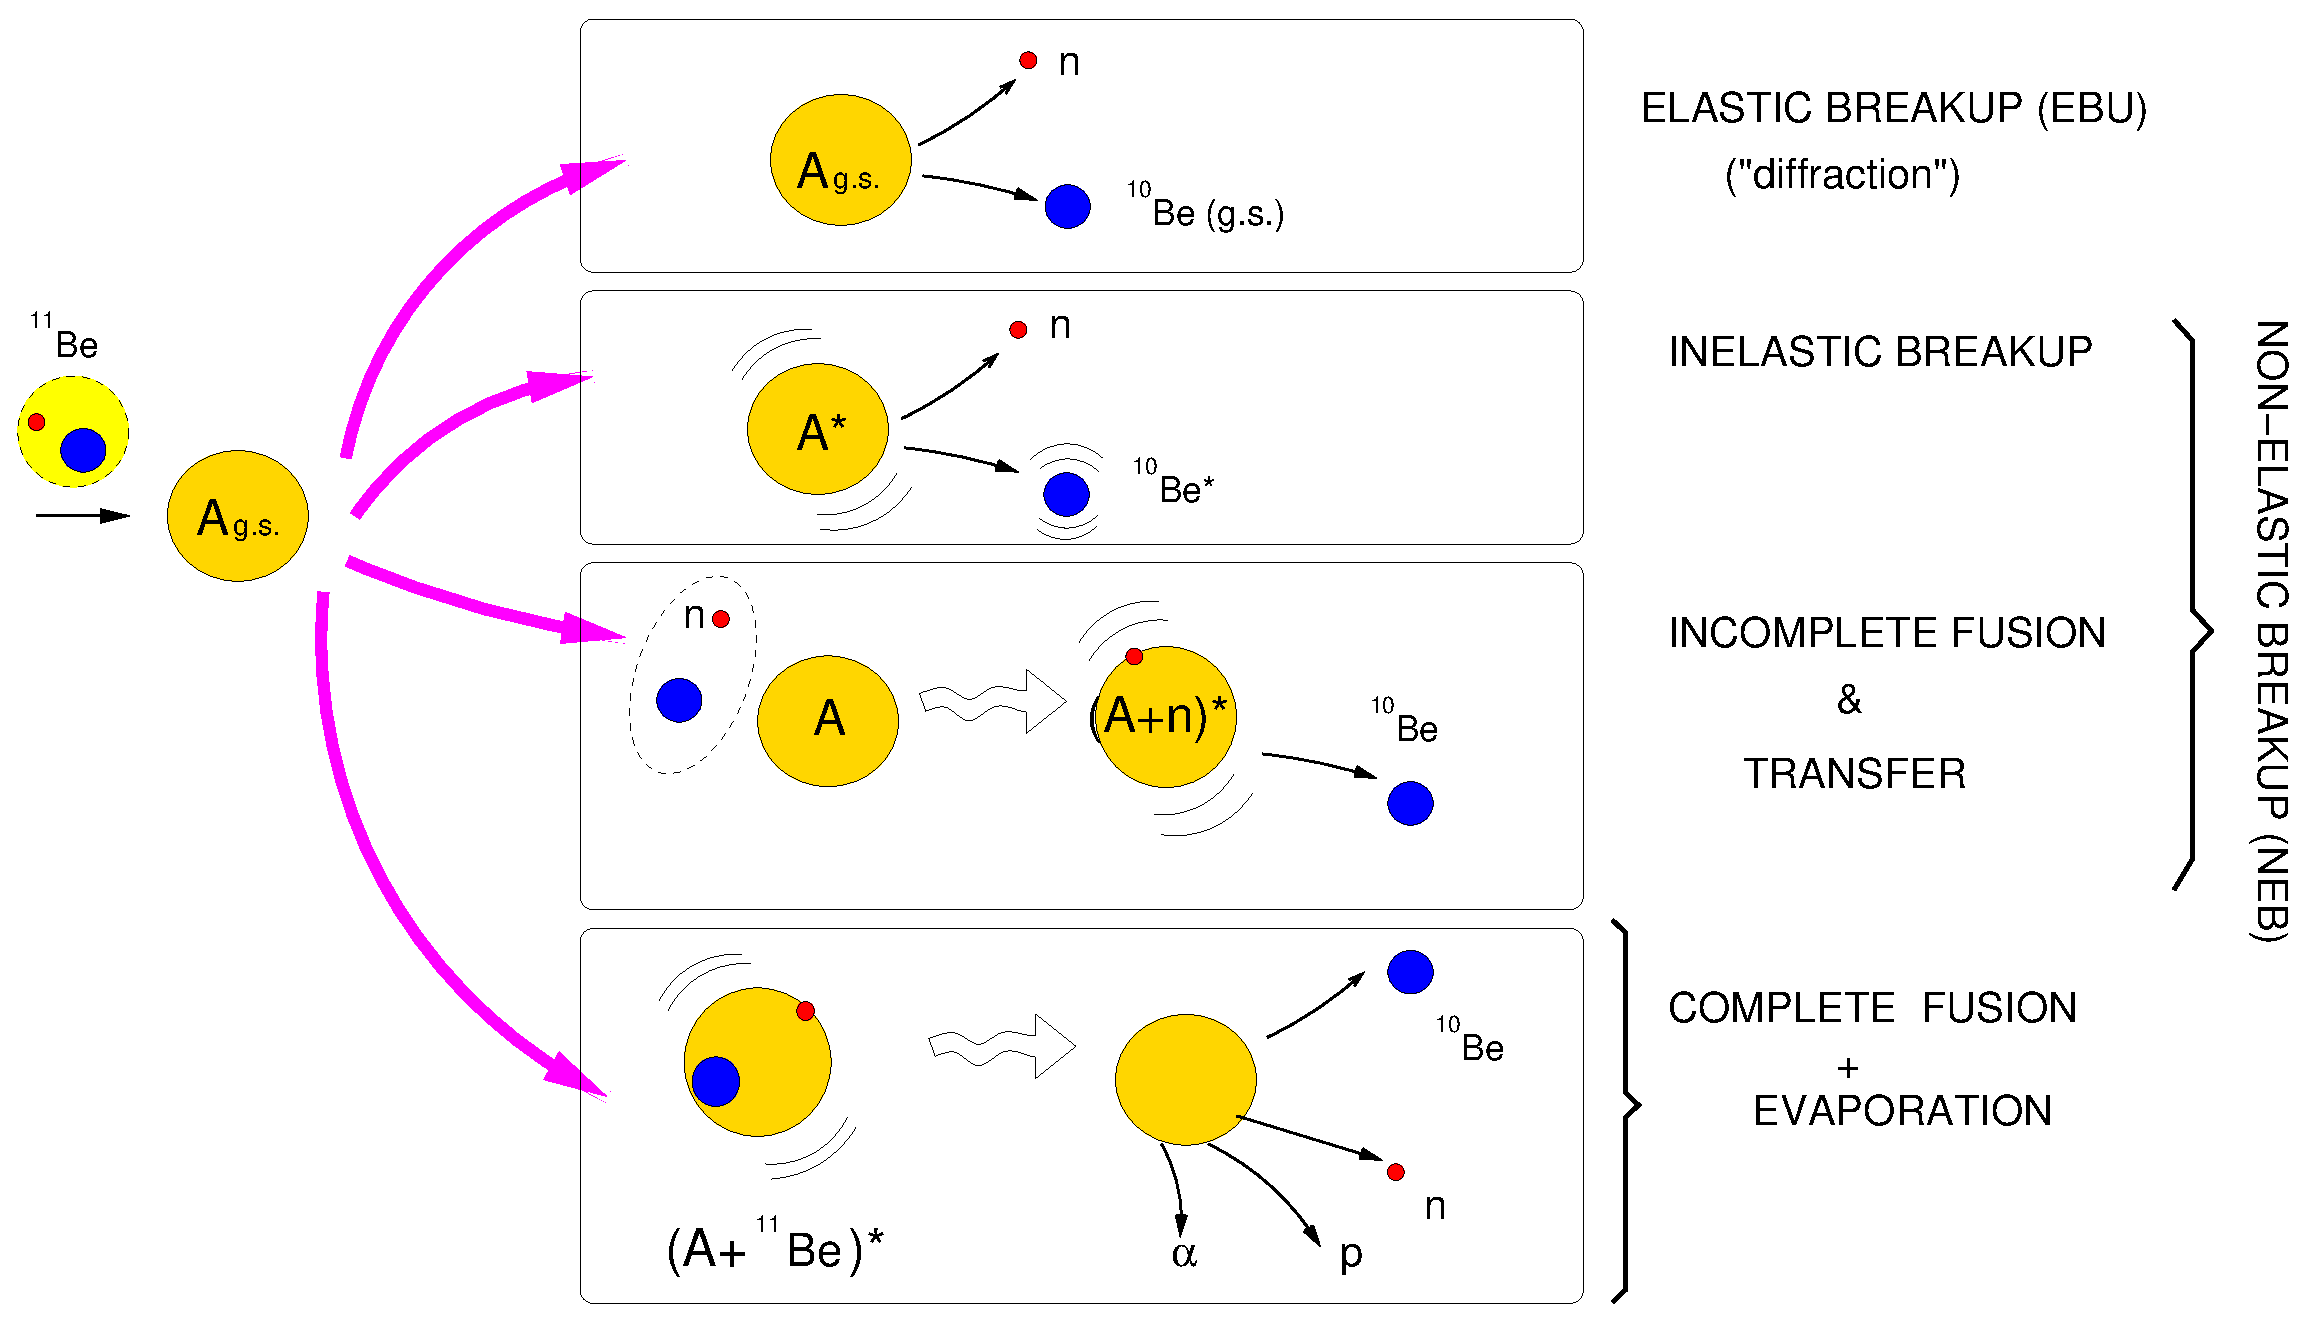
\includegraphics[height=4.5cm]{\images/be11_chans.eps}\end{center}
\column{0.4\textwidth}
\only<2->{
\begin{center} 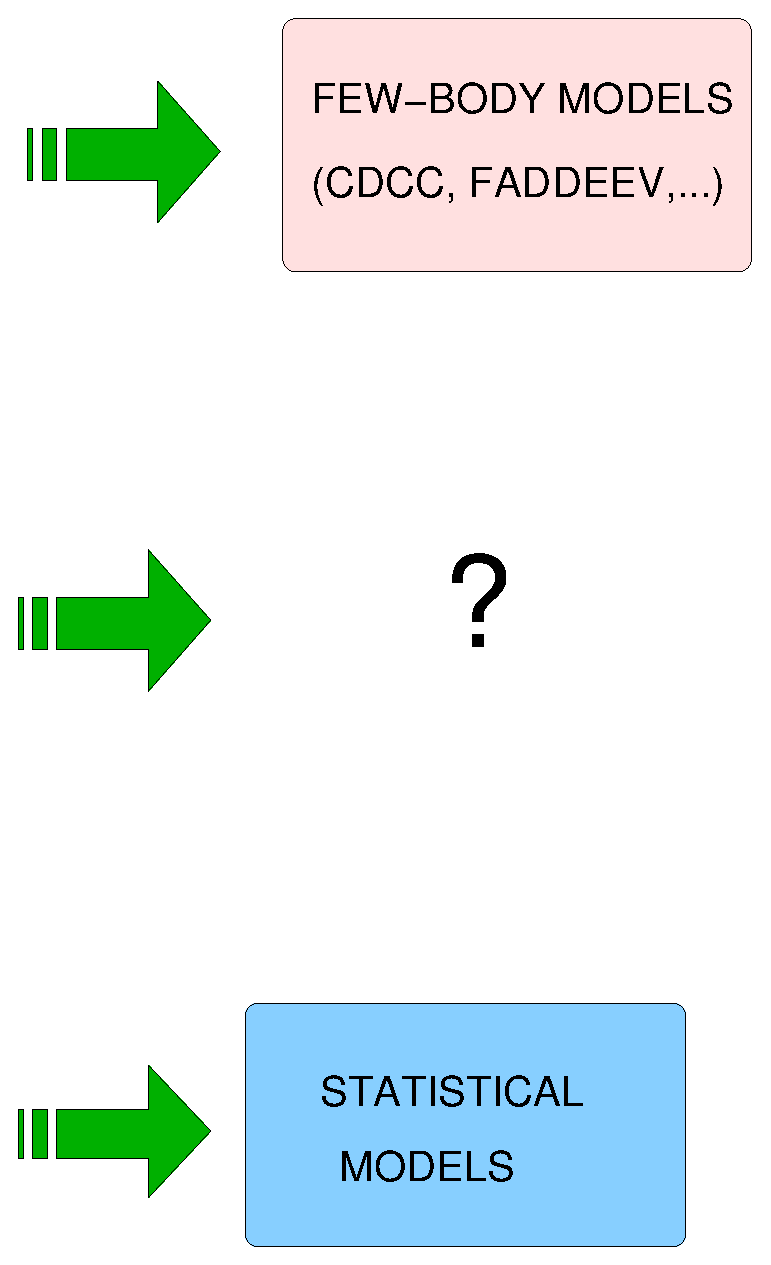
\includegraphics[height=4.5cm]{\images/be11_methods.eps} \end{center}
}%only
\end{columns}
\end{center}
\vspace{0.3cm}

\begin{itemize}
\small
\item [\ding{233}]{\small  For a reaction of the form  $a(=b+x)  + A \rightarrow b + \textrm{anything}$ }
$$
%\psframebox[linecolor=red,framearc=0.25,framesep=0.1cm]{
\psframebox[linecolor=red,fillcolor=orange!10,fillstyle=solid,framearc=0.2]{
\sigma_b =  \sigma_{EBU} + \sigma_{NEB} + \sigma_{CN} 
}
$$  
\item[\ding{233}] {\small CDCC provides only the EBU part ($\sigma_{NEB}$ \& $\sigma_{CN}$ out of CDCC modelspace}
\end{itemize}
\end{frame}




%------------------------------------------------------------------------
\slide{Evidence of NEB contributions in inclusive ($^6$Li,$\alpha$X) }

\begin{columns}
\column{0.5\textwidth} %------------------------------------------------------------------------
\psframebox[fillcolor=LightBlue!50,fillstyle=solid,framearc=0.2]{
 \parbox{5cm}{
 \begin{center}{\brick \scriptsize  $^{6}$Li+$^{209}$Bi @ 32 MeV} \\
 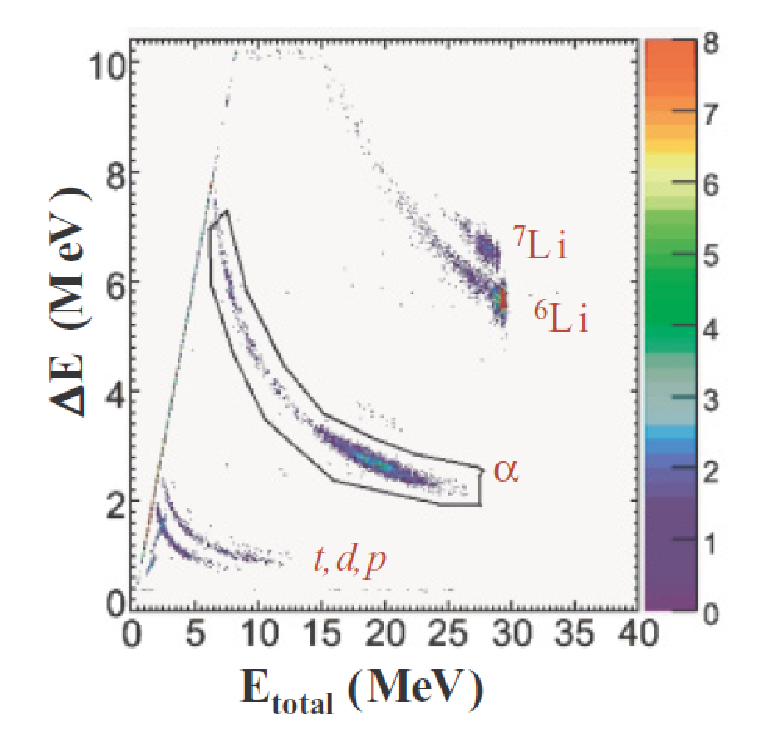
\includegraphics[width=4.5cm]{\images/li6bi_bidim.eps} \\
 \scriptsize
 Santra {\it et al}, PRC85,014612(2008) \end{center}
  }%parbox
 }%psframe
\column{0.5\textwidth} %------------------------------------------------------------------------
If elastic breakup were the dominant mechanism, we would expect $N_\alpha \approx N_{d}$ but,
experimentally, one finds  $N_\alpha \gg N_{d}$
\end{columns}


\end{frame}


%------------------------------------------------------------------------
\slide{Evidence of NEB contributions in inclusive $^{209}$Bi($^6$Li,$\alpha$)X }

\begin{columns}[t]
\column{0.5\textwidth}
\only<1>{
\begin{center}{\brick Elastic scattering} \end{center}
\begin{center}\includegraphics[height=6.0cm]{\images/li6bi_el.eps} \end{center}
%(\scriptsize 3b-CDCC requires reduced d+$^{209}$Bi absorption $\rightarrow$ Ogata's talk)
}%only
\column{0.5\textwidth}
\only<1>{
\begin{center}{\brick Inclusive $\alpha$'s } \end{center}
\begin{center}\includegraphics[height=6.0cm]{\images/li6bi_dsdw_ebu.eps} \end{center}
}%only
\end{columns}
\end{frame}




%-------------------------------------------------------------------------------------------------
\slide{Explicit evaluation of inclusive breakup in Ichimura-Austern-Vincent model}

\bi 
\bitem{Inclusive breakup:} 
$$
\psframebox[linecolor=red,fillstyle=solid,framearc=0.2]{
 a(=b+x) + A \rightarrow b + (x+A)^* 
}%
$$

\psframebox[fillcolor=red!10,framearc=0.2,framesep=4pt]{
\parbox{0.85\columnwidth}{%
{\it  Inclusion of all relevant $x+A$ channels is not feasible in general $\Rightarrow$ use closed-form models}
}%parbox
}%psframe


\bitem{Inclusive differential cross section: $\sigma^\mathrm{BU}_{b} = \sigma^\mathrm{EBU}_b +  \sigma^\mathrm{NEB}_b$}:
\bi
\item $\sigma^\mathrm{EBU}_b$ is breakup leaving $A$ in g.s. (e.g.\ CDCC)
\item  $\sigma^\mathrm{NEB}_b$ corresponds to non-elastic x+A processes and can be calculated as the absorption in the $x+A_{gs}$ channel:
$$
\psframebox[linecolor=red,fillcolor=orange!10,fillstyle=solid,framearc=0.2]{
\frac{d\sigma^\mathrm{NEB}}{d \Omega_b d E_b} = - \frac{2}{\hbar v_a} \rho_b(E_b) \langle \varphi^{(0)}_x | W_{xA} | \varphi^{(0)}_x \rangle
}%psframe
\quad
\textrm{(optical theorem)}
$$

where $\varphi^{(0)}_x$ describes $x-A$ scattering following $a \rightarrow b+x$ dissociation: 
$$
\psframebox[linecolor=red,fillcolor=orange!10,fillstyle=solid,framearc=0.2]{
 [K_x + U_{xA} -E_x] \varphi^{(0)}_{x}(\br_x) = ( \chi_b^{(-)} | V_{bx} | \chi_{aA} \phi_{a}  \rangle
}
$$
\ei

\ei
\end{frame}





%-------------------------------------------------------------------------------------------------
\slide{Application to $^{209}$Bi ($^{6}$Li+,$\alpha$ + X) }
\begin{columns}%[t]
\column{0.5\textwidth}
\begin{center}{\brick Elastic scattering} \end{center}
\begin{center}\includegraphics[height=6.5cm]{\images/li6bi_el.eps} \end{center}

\column{0.5\textwidth}
\begin{center}{\brick Inclusive $\alpha$'s } \end{center}
\begin{center}\includegraphics[height=6.5cm]{\images/li6bi_dsdw_rem.eps} \end{center}
\end{columns}
\end{frame}



%-------------------------------------------------------------------------------------------------
\begin{frame}[t]
\frametitle{\small $^{6}$Li+$^{209}$Bi: incident energy dependence of cross sections}
%Decomposition of the reaction cross section:
\only<1>{ \begin{center}\includegraphics[height=5.0cm]{\images/li6bi_sigedep_1.eps} \end{center} }
\only<2>{ \begin{center}\includegraphics[height=5.0cm]{\images/li6bi_sigedep_2.eps} \end{center} }
\only<3>{ \begin{center}\includegraphics[height=5.0cm]{\images/li6bi_sigedep_3.eps} \end{center} }
\only<4>{ \begin{center}\includegraphics[height=5.0cm]{\images/li6bi_sigedep_4.eps} \end{center} }
\only<5>{ \begin{center}\includegraphics[height=5.0cm]{\images/li6bi_sigedep_5.eps} \end{center} }
\only<6>{ \begin{center}\includegraphics[height=5.0cm]{\images/li6bi_sigedep.eps} \end{center} }

\only<6>{
%Our preliminary calculations indicate that:
$$
\psframebox[linecolor=red,framearc=0.25,framesep=0.1cm]{
\sigma_{reac} \approx \sigma_{\alpha+d} (EBU)+ \sigma_{\alpha}(NBU) + \sigma_{d} (NBU)  + \sigma(CF)
}%psframe
$$
%\ding{43} {\it \verde Suggests small transfer cross sections (for this reaction!)}
}%only

\end{frame}






%--------------------------------------------------------
\slide{Application to the $^{7}$Be case }
%--------------------------------------------------------

Data: Mazzocco {\it et al}:  \ding{43} $\sigma_\alpha \approx 5 \sigma_\mathrm{3He}$

\begin{center}\includegraphics[height=4.5cm]{\images/7Be58Ni.eps} \end{center}

\end{frame}






